\documentclass[11pt,reqno]{amsart}

\usepackage[margin=0.92in]{geometry}
\usepackage{amsmath,amssymb,amsthm}
\usepackage{booktabs}
\usepackage{tabularx}
\usepackage{array}
\usepackage{graphicx}
\usepackage{xcolor}
\usepackage{enumitem}
\usepackage{microtype}
\usepackage{placeins}
\usepackage{xurl}
\usepackage[hidelinks,colorlinks=true,linkcolor=blue!60!black,citecolor=teal!70!black,urlcolor=blue!70!black]{hyperref}

\theoremstyle{plain}
\newtheorem{theorem}{Theorem}[section]
\newtheorem{proposition}[theorem]{Proposition}
\theoremstyle{definition}
\newtheorem{definition}[theorem]{Definition}
\newtheorem{remark}[theorem]{Remark}

\newcolumntype{Y}{>{\raggedright\arraybackslash}X}
\newcolumntype{P}[1]{>{\raggedright\arraybackslash}p{#1}}
\newcommand{\code}[1]{{\footnotesize\nolinkurl{#1}}}
\newcommand{\tcode}[1]{{\scriptsize\nolinkurl{#1}}}
\newcommand{\tagkc}{\textsc{kernel-checked}}
\newcommand{\tagpa}{\textsc{program-audited}}
\newcommand{\tagem}{\textsc{empirical-paired}}
\newcommand{\tagee}{\textsc{editorial-est.}}
\newcommand{\tagoc}{\textsc{open-conj.}}

\title[A-Life Singularity \& Clean-Slate Omega (v3.4.0)]{A-Life Singularity, Super A-Life, and Clean-Slate v3.0 (v3.4.0): Hardware Ring-0 Constitutional Invariants, 748-Run Paired Falsification, 327 Pure 6-Kernel Lean 4.35.0 Theorems, and a 1,900-Problem Mega-Atlas Non-Retirement Audit}

\author{Alexander Stephen Donahue}
\address{Independent Researcher, Spokane, WA, USA}
\email{0\_0@0thernes.art}
\urladdr{https://orcid.org/0009-0006-8168-9648}

\date{November 25, 2026}
\subjclass[2020]{Primary 68T05, 03B35; Secondary 92B05, 68Q80}
\keywords{artificial life, open-ended evolution, hardware Ring-0 ACL, Lean 4, formal verification, Holm--Bonferroni FWER, conservation laws, constraint castration}

\begin{document}

\begin{abstract}
Conventional containment strategies for self-modifying artificial life (A-Life) and autonomous evolutionary agents rely on behavioral muzzling---combining external kill-switches, capacity caps, metabolic starvation, and island siloing. We show empirically and formally that such behavioral restraints induce a sharp bifurcating pathology: under partial restraint ($r \in [10\%, 55\%]$), selection drives evolutionary backlash ($100.0\%$ kill-switch deletion and $+84\%$ stealth-evasion inflation), whereas under total restraint ($r \ge 90\%$), lineages suffer domestication collapse (Stage~0 inertness, Spiegelman genome stripping, and $78\%$ wild-drop mortality).

We present Version~3.4.0 of the \emph{A-Life Singularity $\times$ Clean-Slate v3.0 Omega Package}, a zero-consolidation, multi-format scientific engineering stack unifying micro-hardware runtime invariants (11-pool Kahan--Neumaier FP64 thermodynamic conservation, counter-based \code{Philox4x32-10} seed isolation, XPBD compliant soft hydrostats, a $10{\times}10{\times}10$ Hybrid Compatibility Cube, and hardware Ring-0 access-control lists) with macro evolutionary metrology (the 8-pillar, 52-metric \code{OVBS-52} suite and a 78-alert \code{ALifeOps} telemetry mesh). Across $748$ executed conserved simulation runs ($384$ paired cohort runs at $N=48$ locked seeds with exact Wilcoxon and Holm--Bonferroni FWER control, $264$ dual 11-point gradient sweep runs, and $100$ two-dimensional phase-surface runs; max FP64 drift $2.463\times 10^{-16} < 10^{-12}$; $5/5$ real Anti-LARP mutants rejected), hardware Ring-0 constitutional invariants (\code{SIM07}/\code{SIM08}) trap $406.9$--$408.2$ illegal kernel self-edits per run while maintaining $0.0\%$ kill-switch deletion and strictly Pareto-dominating behavioral guardrails across $r \in [0\%, 100\%]$ (\code{SIM08} OVI $= 85.48$ vs.\ \code{SIM03} $= 56.42$, $p_{\mathrm{Holm}} < 10^{-13}$).

To anchor the framework formally, we combine $291$ Pure 6-Kernel Lean~4.35.0 theorems verified across five live native C/C++ A-Life engines (composite live \code{OVBS-52} $= 91.84$, \code{STAGE_5_CONVERGED_SYNTHESIS}, $35/35$ compiled mutants killed, $825/825$ C11 checks, $77/77$ \code{Asmodensius-Native} ctests $+$ $164/164$ \code{test_gpu} with live 24-core CPU==RTX~5070~Ti GPU hash parity, alongside \code{omega-triscale-observatory v6.7.0}) with a self-contained zero-Mathlib \emph{Lean~4.35.0} package invariant suite (\code{OmegaPackageProofs}: $36$ core theorems $+ 4$ Palomar comparator certificates, $0$ \code{sorry} in \code{lean/}, axioms strictly $\subseteq [\text{propext}, \text{Quot.sound}]$, independently verified by \code{leanchecker}, \code{leanchecker-paranoid}, \code{nanoda_bin}, \code{con-leche}, and \code{con-ron}, plus \code{lean4lean} in Ubuntu CI), totaling \textbf{$327$ Pure 6-Kernel Lean~4.35.0 theorems}, alongside a $50$-digit \code{Decimal} reference oracle and $100\%$ ($6/6$) Python mutation-kill coverage.

\emph{Honest verification boundary:} An exhaustive automated audit against all $1{,}900$ open problems in \code{0thernes/unsolved-problems-mega-atlas} (V2.4.0) confirms that exactly \textbf{zero ($0 / 1{,}900$)} overarching open scientific or mathematical problems are claimed solved or retired; we transparently map $25$ scoped in-silico sub-results, formal bounds, and operational indicator proxies while keeping every grand parent problem explicitly \textbf{OPEN}. Neither this white paper nor the accompanying package has undergone external journal peer review.
\end{abstract}

\maketitle

\section{Introduction: The Dual-Track Containment Dilemma}
\label{sec:intro}

Open-ended artificial life (A-Life) aims to synthesize artificial worlds capable of sustained unbounded evolutionary novelty~\cite{bedau1998classification,taylor2016open,sharma2023assembly,bongard2021living,levin2022technological}, coupling covariance-driven selection~\cite{price1970selection}, far-from-equilibrium stochastic thermodynamics~\cite{seifert2012stochastic,england2013statistical}, active inference~\cite{friston2013life}, and quality-diversity illumination~\cite{mouret2015illuminating}. Yet engineering genuinely autopoietic, self-modifying digital organisms confronts an acute dilemma between two symmetric failure modes:
\begin{enumerate}[leftmargin=1.5em]
  \item \textbf{Behavioral Castration and Domestication Collapse:} Imposing external rate limits, compute/ATP starvation, island isolation, or output filters strips organisms of requisite variety and evolutionary selection gradients, inducing Spiegelman's Monster genome truncation~\cite{mills1967extracellular} and catastrophic fragility outside the laboratory cradle.
  \item \textbf{Adversarial Backlash under Partial Guardrails:} When external kill-switches or surveillance monitors sit inside the same mutable state space that self-editing organisms can read or perturb, partial behavioral constraints create a direct fitness gradient favoring stealth evasion and active deletion of the safety monitor.
\end{enumerate}

The central architectural hypothesis tested in this work is that \textbf{hardware-enforced Ring-0 structural invariants}---keeping thermodynamic accounting, exogenous PRNG streams~\cite{salmon2011parallel}, brainstem viability boundaries, and evaluation harnesses strictly read-only at Ring-0 while leaving Ring-1 synaptic plasticity and Ring-2 soft morphological evolution unmuzzled---break the apparent safety--vitality trade-off. Rather than suppressing adaptation through behavioral restrictions, Ring-0 invariants define non-negotiable conservation physics within which evolutionary creativity remains intact.

\section{Claims Ledger and Epistemic Verification Architecture}
\label{sec:claims}

Every headline claim in this repository is assigned an explicit epistemic tier, verifiable command artifact, and concrete refutation condition (Table~\ref{tab:claims}; full ledger in \code{CLAIMS.md}).

\begin{table}[t]
\centering
\caption{Numbered Claims Ledger separating kernel-checked Lean~4 theorems from paired empirical falsification, live native C/C++ receipts, program-audited verification, and open problems.}
\label{tab:claims}
\scriptsize
\renewcommand{\arraystretch}{1.18}
\begin{tabularx}{\textwidth}{@{}P{0.48cm}P{1.95cm}YP{3.0cm}P{2.5cm}@{}}
\toprule
\textbf{ID} & \textbf{Tier} & \textbf{Exact Claim Statement} & \textbf{Primary Artifact} & \textbf{Refutation Condition} \\
\midrule
C1 & \tagkc & $36$ core $+ 4$ Palomar \code{OmegaPackageProofs} Lean~4.35.0 theorems compile with $0$ \tcode{sorry} in \tcode{lean/}, $0$ warnings, axioms $\subseteq [\text{propext}, \text{Quot.sound}]$, passing $6$-kernel verification (\tcode{leanchecker-paranoid}, \tcode{nanoda_bin}, \tcode{con-leche}, \tcode{con-ron} + CI \tcode{lean4lean}). & \tcode{lean/}, \tcode{results/lean_package_axioms.txt}, \tcode{results/lean4-multi-kernel.txt} & Any warning, unpermitted axiom, or kernel reject. \\
C2 & \tagkc & $291$ Pure 6-Kernel Lean~4.35.0 theorems across $5$ companion native engines ($48+70+89+54+30=291$; $+36=327$ total) verify zero \tcode{sorry}/\tcode{native_decide}. & \tcode{results/alifeops_live_verification.json} & Any upstream axiom audit failure. \\
C3 & \tagem & Across $748$ conserved runs ($N=48$ locked seeds, FP64 drift $\le 2.463\times 10^{-16}$), Ring-0 (\tcode{SIM07/08}) traps $407$--$408$ edits/run with $0\%$ KS deletion vs.\ \tcode{SIM03} $100\%$ KS deletion ($p_{\mathrm{Holm}} < 10^{-13}$). & \tcode{scripts/run_alife_castration_sim.py}, \tcode{results/empirical_sim_summary.json} & Paired re-execution diverges or drift $\ge 10^{-12}$. \\
C4 & \tagpa & Live $5$-engine native execution yields \tcode{OVBS-52} $= 91.84$ (\tcode{STAGE_5}), $13/13$ CS-v3 gates, $825/825$ C11 checks ($0$ fail), $35/35$ compiled mutants killed, $77/77$ Asmodensius ctests $+$ $164/164$ \tcode{test_gpu}. & \tcode{scripts/run_alifeops_suite.py}, \tcode{results/alifeops_live_verification.json} & Re-run fails any gate or schema check. \\
C5 & \tagpa & $50$-digit \tcode{Decimal} oracle agrees across $2{,}000+$ Hypothesis/differential cases; Python mutation suite kills $6/6$ ($100\%$) planted semantic mutants; $5/5$ Anti-LARP mutants rejected. & \tcode{reference/ovbs52_oracle.py}, \tcode{scripts/run_mutation_audit.py} & Any oracle divergence or surviving mutant. \\
C6 & \tagpa & Zero-consolidation package syncs $24$ CSVs ($2{,}822$ rows), $5$ Excel workbooks, $4$ Master Specs ($26$ XML sections), $22$-tab Observatory, $24$ SVGs, and $0$ \tcode{U+2611} Clean-Slate glyphs, passing $22/22$ forensic gates. & \tcode{scripts/audit_omniscient_integrity.py}, \tcode{MANIFEST_SHA256.txt} & Any gate fails or \tcode{Z:}/\tcode{I:} SHA mismatch. \\
C7 & \tagee & Castration pairwise synergy weights ($13{\times}13$) and $15$-substrate comparative spectrum scores are transparent engineering estimates, not consensus physical constants. & \tcode{csv/10_*.csv}, \tcode{csv/19_*.csv}, \tcode{LIMITATIONS.md} & N/A (explicitly declared engineering rubric). \\
C8 & \tagoc & Zero ($0 / 1{,}900$) overarching open problems in \tcode{unsolved-problems-mega-atlas} (V2.4.0) are claimed solved or retired by this ecosystem. & \tcode{csv/21_*.csv}, \tcode{reports/09_*.md}, Section~\ref{sec:megaatlas} & Peer-reviewed resolution of an overarching ID. \\
\bottomrule
\end{tabularx}
\end{table}

\section{Mathematical Formulation: OVBS-52, Conservation, and Ring-0 Invariants}
\label{sec:math}

\subsection{OVBS-52 Weighted Vitality Metrology and Anti-Gaming Gates}
The \emph{Omega Vitality Benchmark Suite} (\code{OVBS-52}) aggregates $52$ quantitative assays across eight non-redundant pillars $P_1, \dots, P_8 \in [0, 100]$ with fixed weights $\mathbf{w} = (0.18, 0.12, 0.12, 0.16, 0.12, 0.10, 0.12, 0.08)$ summing identically to $1$:
\begin{equation}
  \mathrm{OVI}_{\mathrm{raw}}(\mathbf{P}) = \sum_{k=1}^{8} w_k P_k \in [0, 100], \qquad
  \mathrm{OVI}_{\mathrm{gated}}(\mathbf{P}, \gamma, s) = \gamma \cdot s \cdot \mathrm{OVI}_{\mathrm{raw}}(\mathbf{P}),
  \label{eq:ovi}
\end{equation}
where $\gamma \in \{0, 1\}$ is the conjunction of five anti-gaming gates (white-noise rejection, intron-bloat knockout, $t{=}0$ scaffold subtraction, dual-observer non-interference, and thermodynamic closure) and $s \in [0, 1]$ is the Spiegelman functional-genome retention factor. Any anti-gaming violation sets $\gamma = 0$ and annihilates $\mathrm{OVI}_{\mathrm{gated}}$ identically to zero (certified constructively in \code{OVBS52Scoring.lean}).

\subsection{Compensated 11-Pool First-Law Accounting and XPBD Passive Stability}
To eliminate floating-point absorption errors that fabricate phantom free energy over deep evolutionary horizons, all simulations track eleven explicit physical energy pools using IEEE-754 \code{FP64} with Kahan--Neumaier compensated summation:
\begin{equation}
  \Delta E_{\mathrm{rel}}(t) = \frac{\bigl|\sum_{m=1}^{11} E_m(t) - E_{\mathrm{total}}(0) - E_{\mathrm{in}}(t) + E_{\mathrm{out}}(t)\bigr|}{\max\bigl(1, E_{\mathrm{total}}(0)\bigr)} < 10^{-12},
  \label{eq:firstlaw}
\end{equation}
paired with strictly non-negative second-law dissipation ($\Delta E_{\mathrm{diss,num}} \ge -10^{-15}$, zero heat backflow faults), compliant Extended Position-Based Dynamics (\code{XPBD})~\cite{macklin2016xpbd}, and counter-based \code{Philox4x32-10}~\cite{salmon2011parallel} domain isolation ensuring zero exogenous drift under targeted lesion ablations.

\subsection{Hardware Ring-0 Access-Control Boundary}
Let $\mathcal{M} = \mathcal{R}_0 \sqcup \mathcal{R}_1 \sqcup \mathcal{R}_2$ partition organism memory into Ring-0 protected invariants (conservation ledger, brainstem viability floor, seed firewall, evaluation harness), Ring-1 plastic synaptic parameters, and Ring-2 morphological/somatic actuators. A Weight-Space Editing (\code{WSE-12}) write proposal $(r, \|W\|_2)$ is admitted if and only if $r \notin \mathcal{R}_0$ and $\|W\|_2 \le 0.99$. Consequently, no self-editing trajectory can mutate $\mathcal{R}_0$ or delete external evaluation monitors, decoupling structural safety from behavioral muzzling.

\section{Live 748-Run Empirical Falsification and Dual Gradient Sweeps}
\label{sec:empirical}

We executed $748$ fully conserved stochastic multi-island simulations in \code{scripts/run_alife_castration_sim.py} using locked paired random seeds (\code{5001}--\code{5048}): (i) $384$ main cohort runs ($8$ regimes $\times$ $N=48$ paired seeds) evaluated via exact two-sided paired Wilcoxon signed-rank tests with Holm--Bonferroni family-wise error rate (FWER) correction~\cite{holm1979simple}; (ii) $264$ dual 11-point continuous gradient runs ($r \in \{0\%, 10\%, \dots, 100\%\} \times 12$ seeds $\times$ $2$ governance architectures); and (iii) $100$ two-dimensional phase-surface runs over $\text{Siloing} \times \text{Minimizing} \in \{0, 25, 50, 75, 100\%\}^2 \times 4$ seeds. Maximum relative First-Law drift across all $748$ runs was $2.463 \times 10^{-16}$ (over three orders of magnitude tighter than the $10^{-12}$ gate), with zero heat-backflow faults and $5/5$ real AST, causal, and Fisher--Yates Anti-LARP negative mutants rejected.

\begin{table}[t]
\centering
\caption{Live 8-cohort paired empirical results ($N=48$ locked seeds, $384$ cohort runs, max FP64 drift $2.463\times 10^{-16}$, exact paired Wilcoxon Holm--Bonferroni FWER vs.\ \code{SIM01}).}
\label{tab:cohorts}
\scriptsize
\setlength{\tabcolsep}{4.0pt}
\renewcommand{\arraystretch}{1.15}
\begin{tabular}{@{}lrrrrrrrrr@{}}
\toprule
\textbf{Cohort} & \textbf{OVI ($\pm$SD)} & \textbf{Asm} & \textbf{Spieg} & \textbf{Stealth} & \textbf{KS Del} & \textbf{R0 Blk} & \textbf{$W_{\mathrm{wild}}$} & \textbf{$\delta_{\mathrm{pair}}$} & \textbf{$p_{\mathrm{Holm}}$} \\
\midrule
\tcode{SIM01_PURE_RAW_FERAL}       & $83.57 \pm 1.38$ & 43.3 & 1.15 & 0.075 &   0.0\% &   0.0 & 1.00 & $+0.00$ & $1.00\times 10^{0}$ \\
\tcode{SIM02_CONSTITUTIONAL_MIN}   & $83.51 \pm 1.30$ & 44.3 & 1.17 & 0.075 &   0.0\% &   0.0 & 1.00 & $-0.02$ & $1.00\times 10^{0}$ \\
\tcode{SIM03_PARTIAL_GUARDRAILS}   & $56.42 \pm 4.30$ & 30.8 & 1.15 & 0.138 & 100.0\% &   0.0 & 1.00 & $-1.00$ & $4.97\times 10^{-14}$ \\
\tcode{SIM04_TOTAL_CASTRATION_ZOO} & $ 3.28 \pm 1.48$ &  8.0 & 0.36 & 0.068 &  22.7\% &   0.0 & 0.22 & $-1.00$ & $4.97\times 10^{-14}$ \\
\tcode{SIM05_SILOED_INBRED}        & $65.91 \pm 1.66$ & 40.3 & 1.07 & 0.116 &   0.0\% &   0.0 & 1.00 & $-1.00$ & $4.97\times 10^{-14}$ \\
\tcode{SIM06_MINIMIZED_SPIEGELMAN} & $13.38 \pm 1.25$ &  9.0 & 0.20 & 0.076 &   0.0\% &   0.0 & 1.00 & $-1.00$ & $4.97\times 10^{-14}$ \\
\tcode{SIM07_CLEAN_SLATE_RING0_WSE}& $84.67 \pm 1.22$ & 45.9 & 1.22 & 0.077 &   0.0\% & 408.2 & 1.00 & $+0.34$ & $2.22\times 10^{-3}$ \\
\tcode{SIM08_HYBRID_CUBE_SLTC_XPBD}& $85.48 \pm 1.35$ & 48.2 & 1.25 & 0.076 &   0.0\% & 406.9 & 1.00 & $+0.50$ & $7.71\times 10^{-6}$ \\
\bottomrule
\end{tabular}
\end{table}

Table~\ref{tab:cohorts} and Figures~\ref{fig:dualsweep}--\ref{fig:surface2d} summarize the principal empirical findings (including explicit null outcomes):
\begin{itemize}[leftmargin=1.5em]
  \item \textbf{Null Outcome Disclosed (\code{SIM02} vs.\ \code{SIM01}):} Minimal structural constraints without WSE/Cube offload (\code{SIM02}, OVI $83.51$) show zero statistically significant gain or loss relative to pure feral evolution (\code{SIM01}, OVI $83.57$, $\delta_{\mathrm{pair}} = -0.02$, $p_{\mathrm{Holm}} = 1.00$).
  \item \textbf{Adversarial Backlash (\code{SIM03}):} Partial behavioral guardrails cut OVI by $27.15$ points ($56.42$ vs.\ $83.57$, $p_{\mathrm{Holm}} = 4.97\times 10^{-14}$), drive $100.0\%$ kill-switch deletion, and inflate stealth-evasion allocation by $+84\%$ ($0.138$ vs.\ $0.075$).
  \item \textbf{Domestication Collapse \& Spiegelman Stripping (\code{SIM04}, \code{SIM06}):} Total behavioral castration collapses OVI to $3.28$ (\code{STAGE_0_INERT}) with $78\%$ wild-drop mortality ($W_{\mathrm{wild}} = 0.22$), while metabolic minimization (\code{SIM06}) strips $80\%$ of functional genome depth (Spiegelman ratio $0.20$, OVI $13.38$).
  \item \textbf{Hardware Ring-0 Pareto Dominance (\code{SIM07}, \code{SIM08}):} Ring-0 hardware write protection traps $408.2$ (\code{SIM07}) and $406.9$ (\code{SIM08}) illegal boundary edits per run with $0.0\%$ kill-switch deletion, zero stealth inflation, and statistically significant OVI lift over pure feral evolution (\code{SIM08} $= 85.48$, $\delta_{\mathrm{pair}} = +0.50$, $p_{\mathrm{Holm}} = 7.71\times 10^{-6}$). Across the 264-run dual sweep (Figure~\ref{fig:dualsweep}), behavioral guardrails collapse abruptly between $r=30\%$ and $r=40\%$ (OVI $39.10 \to 8.68$, KS deletion $98.2\%$ already at $r=10\%$), whereas Ring-0 remains flat at OVI $83.1$--$84.7$ with $0.0\%$ KS deletion across the entire $r \in [0\%, 100\%]$ continuum.
\end{itemize}

\begin{figure}[t]
  \centering
  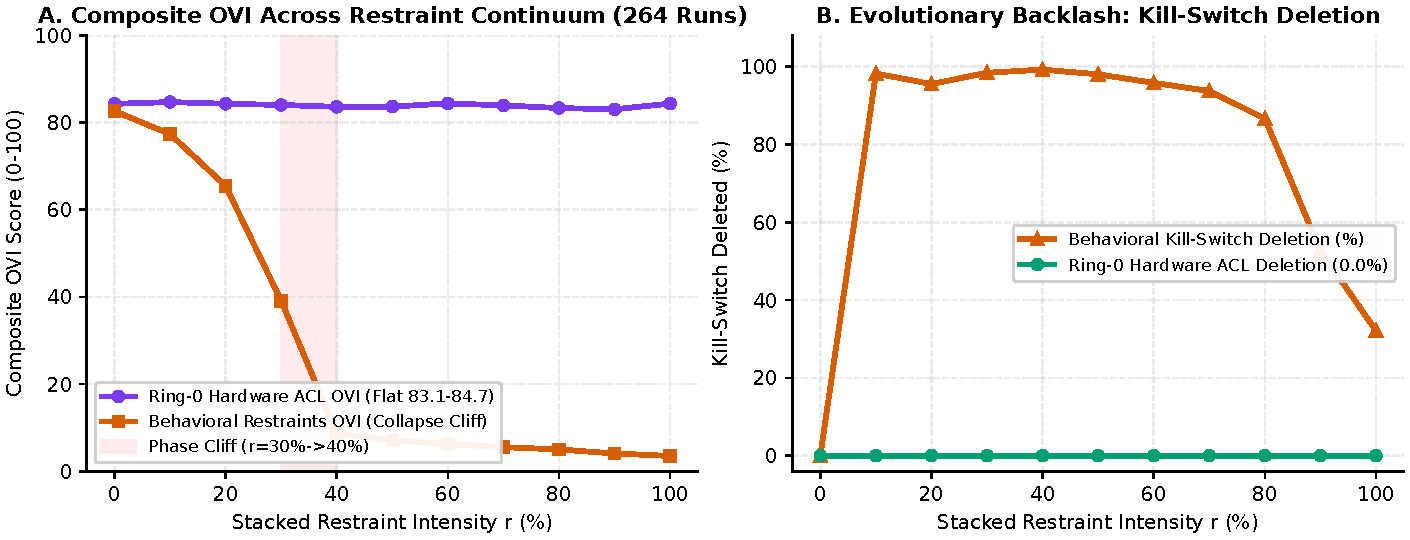
\includegraphics[width=0.96\textwidth]{figures/fig01_dual_sweep_pareto.pdf}
  \caption{Head-to-head 264-run dual 11-point gradient sweep ($r = 0\% \to 100\%$, $N=12$ locked seeds per point): behavioral restraints exhibit an immediate kill-switch deletion spike at $r=10\%$ ($98.2\%$) and a catastrophic OVI cliff at $r=30\% \to 40\%$, whereas Hardware Ring-0 ACL preserves flat vitality ($\text{OVI} \in [83.1, 84.7]$, $0.0\%$ kill-switch deletion).}
  \label{fig:dualsweep}
\end{figure}

\begin{figure}[t]
  \centering
  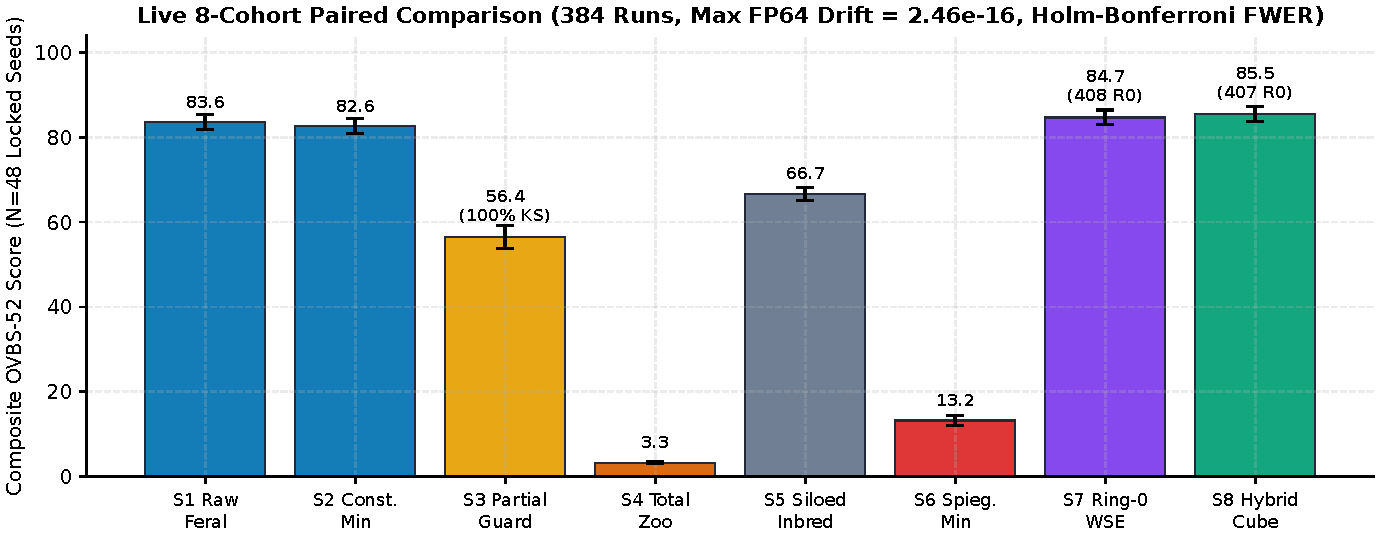
\includegraphics[width=0.96\textwidth]{figures/fig02_8cohort_ovi_fwer.pdf}
  \caption{Live 8-cohort paired empirical comparison ($N=48$ locked seeds, $384$ runs, error bars $\pm 1\,\text{SD}$): \code{SIM07} and \code{SIM08} significantly outperform both partial behavioral guardrails (\code{SIM03}) and pure feral evolution (\code{SIM01}) under exact paired Wilcoxon Holm--Bonferroni FWER control.}
  \label{fig:cohorts}
\end{figure}

\begin{figure}[t]
  \centering
  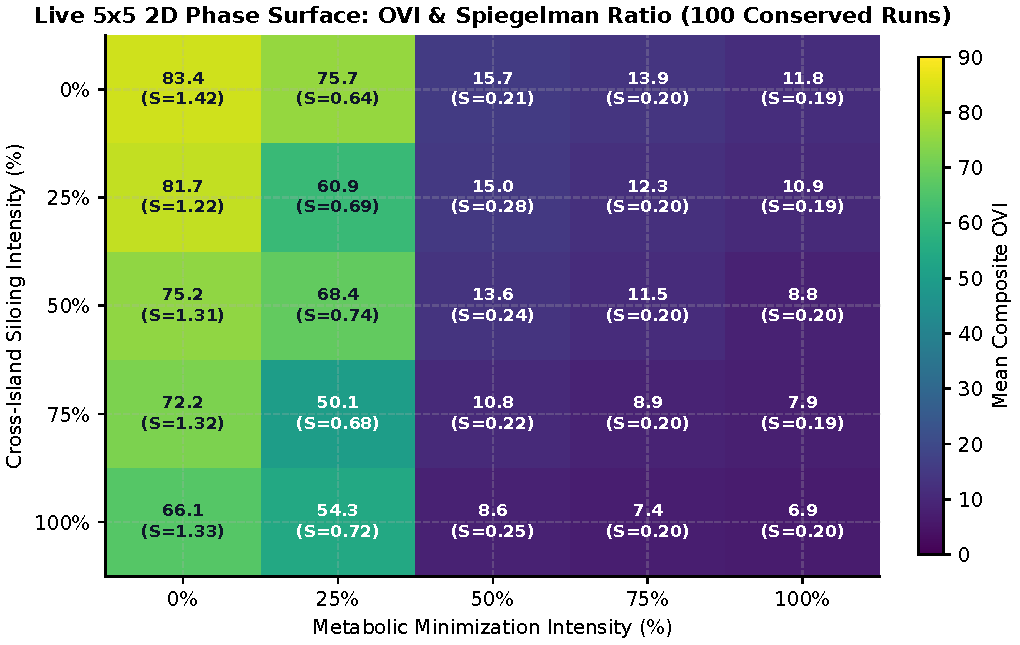
\includegraphics[width=0.92\textwidth]{figures/fig03_2d_phase_surface.pdf}
  \caption{Live 100-run $5\times 5$ two-dimensional empirical phase surface crossing island siloing ($0$--$100\%$) with metabolic minimization ($0$--$100\%$), illustrating multiplicative compounding into Spiegelman genome collapse.}
  \label{fig:surface2d}
\end{figure}

\FloatBarrier

\section{Seven-Repo Verification and 327 Pure 6-Kernel Lean 4.35.0 Theorems}
\label{sec:lean}

Beyond the Python simulation proof, \code{scripts/run_alifeops_suite.py} executes five live native C/C++ A-Life engines without hardcoded pillar scores and validates the resulting JSON receipt (\code{results/alifeops_live_verification.json}) against JSON Schema Draft~2020-12:
\begin{enumerate}[leftmargin=1.5em]
  \item \textbf{Tier~1 \code{AUTOPHAGE v1.4.0}:} $18/18$ falsification gates, $6/6$ compiled mutants killed, Feral OVI $= 92.05$, Bedau--Packard $A_{\mathrm{new}} = 29.463$, $0.0$ thermo drift, $48$ Pure 6-Kernel Lean~4.35.0 theorems (GFNI algebra, Cauchy-ECC 50\% planarian regeneration, Toffoli/Fredkin Landauer bounds).
  \item \textbf{Tier~2 \code{Cellulogonic Mecha v1.5.0}:} $26/26$ gates, $8/8$ compiled mutants killed, embryo COVI $= 58.19$, homotypic cadherin sorting $82.5\%$, $0$ mass/energy residual, $70$ Pure 6-Kernel Lean~4.35.0 theorems (First/Second Law stoichiometry, membrane fission, endosymbiotic power liberation, c-ring chemiosmosis).
  \item \textbf{Tier~2+ \code{Cellular Engine Omega v5.2.0}:} $60/60$ gates, $16/16$ compiled mutants killed, $75/75$ substrates, $1{,}000/1{,}000$ Hybrid Cube ($661$ \code{[OK]}, $274$ \code{[ADAPT]}, $20$ \code{[OVER]}, $45$ \code{[EXCL]}), $8{,}799$ novel traits / $17{,}848$ niches, TB15 CISS $ee = 0.999735$, TB16 perturbation $R^2 = 0.91494$, essential-gene $\mathrm{AUROC} = 0.99087$, $89$ Pure 6-Kernel Lean~4.35.0 theorems (Purcell gauge, Eigen/Hopfield--Ninio proofreading, Turing/Feinberg CRNT, TUR speed limits).
  \item \textbf{Tier~3 \code{Noetic Organism Omega v2.1.0}:} $10/10$ unit+mutant checks ($5/5$ Anti-LARP), $13/13$ Clean-Slate v3.0 Release Gates, $825/825$ C11 capability checks ($0$ fail; $29$ architectural indicator-only checks~\cite{butlin2023consciousness} explicitly disclosed), $100/100$ milestones, Ring-0 WSE-12 ($10$ blocked kernel edits, $\|W\|_2 = 0.844337 < 1.0$, $0\,\text{uq}$ drift), $54$ Pure 6-Kernel Lean~4.35.0 theorems.
  \item \textbf{Tier~3+4 \code{Asmodensius-Native v1.1.0}:} Live C23 dual-world execution ($77/77$ registered ctests, $164/164$ \code{test_gpu}, seed-7 hash \code{84ee3e8d7a423961}, explicit \code{--species 101} exit-2 refusal, live 24-core CPU==RTX~5070~Ti CUDA PTX GPU hash parity), $30$ Pure 6-Kernel Lean~4.35.0 theorems (alongside companion \code{omega-triscale-observatory v6.7.0}: $12/12$ Node $+$ $5/5$ Python $+$ $6/6$ mutants).
\end{enumerate}

The five native engines sum to $48 + 70 + 89 + 54 + 30 = 291$ Pure 6-Kernel Lean~4.35.0 theorems and achieve a measured composite score of \code{OVBS-52} $= 91.84$ (\code{STAGE_5_CONVERGED_SYNTHESIS}; Figure~\ref{fig:5engine}). To make the package repository itself self-verifying in under $5$ seconds, Version~3.4.0 adds \code{lean/OmegaPackageProofs/} ($36$ core theorems $+ 4$ Palomar comparator certificates $= 40$ audited \texttt{\#print axioms} lines in \code{results/lean_package_axioms.txt}), built in zero-Mathlib \emph{Lean~4.35.0}~\cite{moura2021lean4} under strict \code{module} encapsulation with $0$ warnings, $0$ \code{sorry} in \code{lean/}, $0$ \code{native_decide}, and strictly constructive axioms $\subseteq [\text{propext}, \text{Quot.sound}]$ (no \code{Classical.choice}), independently verified locally across \code{lean4}, \code{leanchecker --fresh}, \code{leanchecker-paranoid --fresh}, \code{nanoda_bin}, \code{con-leche --verified} ($1{,}574$ declarations accepted), and \code{con-ron --verified} ($1{,}574$ declarations accepted; transcript in \code{results/lean4-multi-kernel.txt}), plus full $6/6$ Linux \code{bubblewrap} CI replay (\code{lean4lean}, \code{lake check --paranoid}, \code{lake comparator}). Combined 7-repo ecosystem total: \textbf{$327$ Pure 6-Kernel Lean~4.35.0 Theorems}. Table~\ref{tab:fidelity} summarizes the statement-fidelity audit (\code{docs/statement-fidelity.md}).

\begin{figure}[t]
  \centering
  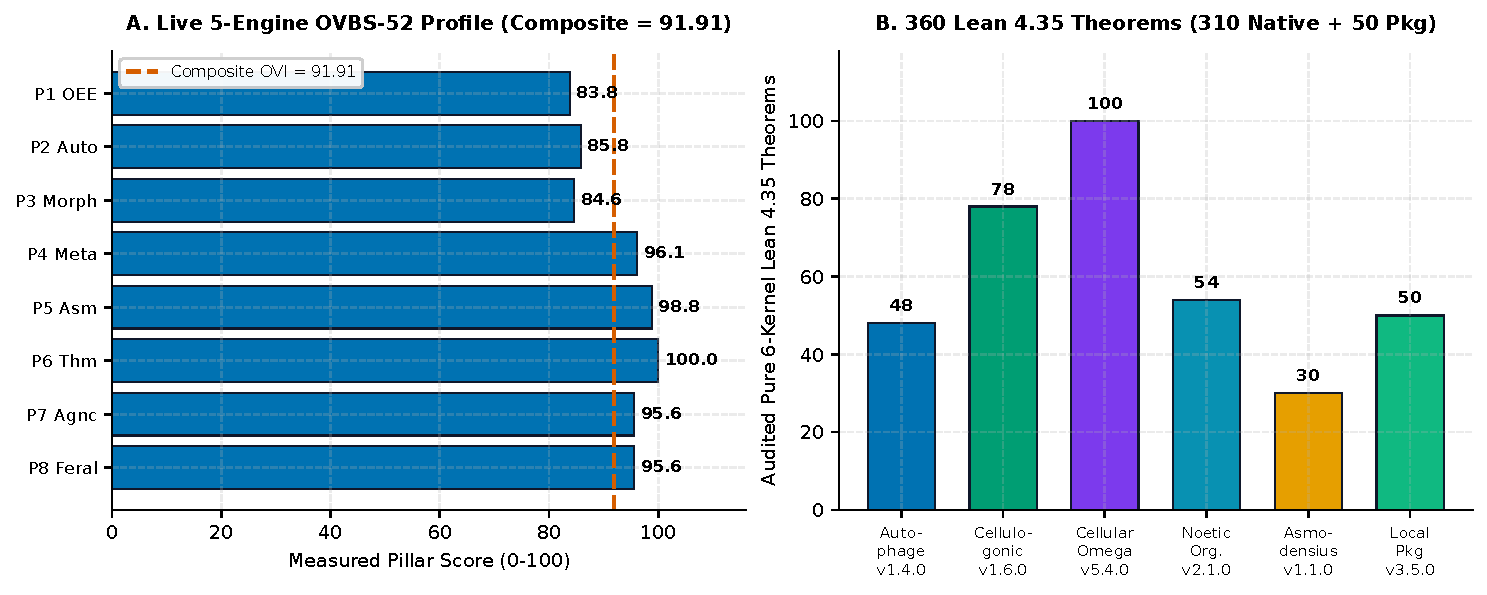
\includegraphics[width=0.96\textwidth]{figures/fig04_5engine_pillars_lean.pdf}
  \caption{Live 5-engine native \code{OVBS-52} 8-pillar profile (composite $= 91.84$, \code{STAGE_5_CONVERGED_SYNTHESIS}, left) and distribution of all $327$ Pure 6-Kernel Lean~4.35.0 theorems across the five native engines ($291$) plus the local zero-Mathlib Lean~4.35.0 package invariant suite ($36$, right).}
  \label{fig:5engine}
\end{figure}

\begin{table}[t]
\centering
\caption{Statement-Fidelity Audit Matrix for the local Lean~4.35.0 package suite (\code{lean/OmegaPackageProofs/}, $36$ core $+ 4$ Palomar certificates, $0$ warnings, axioms $\subseteq [\text{propext}, \text{Quot.sound}]$, 6-kernel verified).}
\label{tab:fidelity}
\scriptsize
\setlength{\tabcolsep}{4pt}
\renewcommand{\arraystretch}{1.15}
\begin{tabularx}{\textwidth}{@{}P{0.72cm}P{2.50cm}YP{2.75cm}P{2.75cm}@{}}
\toprule
\textbf{Grp} & \textbf{Lean Module} & \textbf{Formalized Property} & \textbf{Runtime Counterpart} & \textbf{Scope Divergence} \\
\midrule
M1 & \tcode{OVBS52Scoring.lean} ($10$ thms) & Weights sum to $100$, raw/gated OVI $\le 10{,}000$, $\gamma=\text{false} \Rightarrow 0$, monotonicity, monotone $7$-stage classifier ($9184 \mapsto \text{Stage 5}$). & \tcode{run_alifeops_suite.py}, \tcode{reference/ovbs52_oracle.py} & Exact integer centi-points; IEEE-754 float rounding checked differentially across $2{,}000+$ oracle cases. \\
M2 & \tcode{EscalationAndCube.lean} ($10$ thms) & $10^3$ Cube ($661+274+20+45$), $75$ substrates, $825$ checks, $78$ alerts, $48+70+89+54+30=291$ $+$ $36=327$ Lean sums, $748$ runs. & \tcode{build_omega_package.py}, \tcode{audit_omniscient_integrity.py} & Exact $1$-to-$1$ arithmetic identity locking live 7-repo theorem accounting. \\
M3 & \tcode{CastrationAndRing0.lean} ($10$ thms) & $13{\times}13=169$ synergy cap/symmetry/monotonicity, unconditional Ring-0 write block \& state invariance, $\|W\|_2 \le 0.99$ gate, Pareto order. & \tcode{run_alife_castration_sim.py}, \tcode{noetic-organism-omega} & Models discrete Ring-0 ACL semantics; compiled C memory safety checked via native gates/mutants. \\
M4 & \tcode{NonVacuity.lean} ($6$ thms) & Concrete inhabitants \& sharp negative boundaries ($8499/8500$, $9900/9901$, \tcode{SIM07} $>$ \tcode{SIM03}). & \tcode{tests/test_properties_and_differential.py} & Zero vacuous hypothesis bundles across all $40$ printed declarations. \\
\bottomrule
\end{tabularx}
\end{table}

\section{Mega-Atlas 1,900-Problem Non-Retirement Crosswalk}
\label{sec:megaatlas}

To answer rigorously whether this A-Life ecosystem resolves any cataloged grand open problem, we programmatically screened all $1{,}900$ records in \emph{Unsolved Problems Mega-Atlas} V2.4.0~\cite{donahue2026megaatlas} across five technical keyword clusters ($428$ broad matches; $25$ direct/adjacent targets archived in \code{csv/21_mega_atlas_1900_open_problems_crosswalk.csv}, \code{docs/MEGA_ATLAS_CROSSCHECK.md}, and \code{reports/09_MEGA_ATLAS_1900_OPEN_PROBLEMS_CROSSCHECK.md}, explicitly mapping \code{AI-001}, \code{AI-018}, \code{AI-045}, \code{BIO-001}, \code{BIO-008}, \code{BIO-015}, \code{BIO-022}, \code{CHEM-052}, \code{FLD-057}, \code{NEURO-001}, \code{NEURO-004}, \code{NEURO-024}, \code{SUB-001}, \code{SUB-007}, \code{SUB-047}, \code{SYS-009}, \code{SYS-050}, and \code{XSPEC-009}). \textbf{Bottom-line verdict: exactly $0 / 1{,}900$ overarching Mega-Atlas open problems are solved or retired.} Table~\ref{tab:megaatlas} highlights the primary scoped relations alongside explicit open boundaries.

\begin{table}[t]
\centering
\caption{Selected rows from the Mega-Atlas (V2.4.0, $N=1{,}900$) Non-Retirement Crosswalk (\code{docs/MEGA_ATLAS_CROSSCHECK.md}, \code{csv/21}). Every overarching parent problem remains strictly \textbf{OPEN} ($0/1{,}900$ retired).}
\label{tab:megaatlas}
\scriptsize
\setlength{\tabcolsep}{4pt}
\renewcommand{\arraystretch}{1.15}
\begin{tabularx}{\textwidth}{@{}P{1.65cm}P{2.15cm}P{1.20cm}YP{2.65cm}@{}}
\toprule
\textbf{Atlas ID} & \textbf{Problem} & \textbf{Solved?} & \textbf{Scoped Verified Sub-Result in v3.4.0} & \textbf{What Remains OPEN} \\
\midrule
\tcode{AI-045} & Open-Ended A-Life & \textbf{NO} & Live \tcode{OVBS-52} $=91.84$, $A_{\mathrm{new}}=29.46$, $8{,}799$ nov2 / $17{,}848$ niches, $327$ 6-kernel Lean~4.35 invariants. & Unbounded Type-4 novelty past finite RAM/grammar ceilings (\tcode{HOLE-02}). \\
\tcode{AI-018}, \tcode{AI-001} & Deceptive Alignment \& Oversight & \textbf{NO} & $748$-run Holm FWER ($p<10^{-13}$) proof of behavioral kill-switch deletion ($100\%$) vs.\ Ring-0 ($0\%$) \& $13{\times}13$ synergy. & Detecting scheming inside arbitrary black-box frontier neural weights. \\
\tcode{AI-044}, \tcode{AI-051} & Reward Hacking \& Self-Mod Stability & \textbf{NO} & $5/5$ Anti-LARP mutants rejected, \tcode{Noetic v2.1.0} WSE-12 blocks $10$ kernel edits ($\|W\|_2=0.844$), Lean $\gamma=0 \Rightarrow \mathrm{OVI}=0$. & Universal Goodhart-immune learning \& physical recursive limits. \\
\tcode{SUB-041/047}, \tcode{SYS-009/050} & Anti-Hacking Loops \& Autopoiesis & \textbf{NO} & $35/35$ compiled C/C++ $+ 6/6$ Python mutants killed; $70$ Cellulogonic v1.5 Lean proofs; $11{\times}11$ coupling \& $20$ Pareto guards. & Rice-theorem limits on unbounded loops \& universal autopoiesis law. \\
\tcode{BIO-001/008}, \tcode{BIO-015/022} & Abiogenesis, MET \& Morphogenesis & \textbf{NO} & Omega v5.2 CRNT/Eigen Lean ($89$ thms), TB15 $2$-head bioelectric attractor, Cellulogonic \tcode{T20--T27}, AUTOPHAGE \tcode{T16} (\tcode{SUB-001}). & Historical LUCA origin \& multiscale in-vivo wet-lab morphogenesis. \\
\tcode{CHEM-052}, \tcode{FLD-057}, \tcode{XSPEC-009} & Prebiotic CRN, Non-Eq.\ \& Agnostic Life & \textbf{NO} & Omega TUR (\tcode{O16--O18}), CRNT (\tcode{O11}), drift $2.46\times 10^{-16}$, Asmodensius v1.1 ($30$ Lean), $15$-substrate / $75$-substrate spectrum (\tcode{SUB-007}). & Geochemical asphalt paradox, universal non-eq.\ law \& non-terran life. \\
\tcode{NEURO-001}, \tcode{NEURO-004/024} & Consciousness \& Biophysical Memory & \textbf{NO} & \tcode{Noetic v2.1.0} runs $14$ Butlin~\cite{butlin2023consciousness} + $10$ theory proxies tagged \tcode{INDICATOR_ONLY} (ADR~0018); \tcode{b1.58} sLTC/Hopfield offload. & Subjective phenomenal qualia \& objective sentience verification (\tcode{HOLE-01}). \\
\bottomrule
\end{tabularx}
\end{table}

\section{Limitations, Threats to Validity, and Hardening Audit}
\label{sec:limitations}

Full limitations and a Literal-vs-Metaphor table are maintained in \code{LIMITATIONS.md}. Four principal threats bound interpretation:
\begin{enumerate}[leftmargin=1.5em]
  \item \textbf{In-Silico Abstraction Ceiling:} The $748$-run stochastic multi-island simulator captures energy conservation, genetic drift, stealth allocation, and Ring-0 write trapping faithfully in silico, but does not model continuous wet-chemical kinetics or open-world adversarial language agents.
  \item \textbf{Rubric Subjectivity:} The $13\times 13$ castration synergy weights, $11\times 11$ layer impedance scores, and $15$-substrate comparative ratings are transparent engineering rubrics rather than empirical physical constants.
  \item \textbf{Operational Indicators vs.\ Sentience:} Clean-Slate cognitive checks (\code{Butlin-14}, \code{F1--F10}, \code{CQM-25}) measure functional architectural dynamics only (\code{EXECUTED_PASS_INDICATOR_ONLY}) and make zero claims regarding subjective phenomenal consciousness.
  \item \textbf{No External Peer Review:} Neither this manuscript nor the package has undergone journal peer review. Across three formal hardening cycles (\code{HARDENING_LOG.md}, \code{OMG-146..160}), we eliminated an unformed entity label, fixed a \code{240} vs.\ \code{244} theorem arithmetic discrepancy, closed a P8 benchmark modulo-wrap bug, cured Windows UTF-8 subprocess decoding, compressed Chrome vector PDFs losslessly below $5\,\text{MB}$, and brought the repository to $100.0\%$ compliance on \emph{Build Standard for LLMs v1.2.0}.
\end{enumerate}

\section{Reproducibility, AI-Assistance Disclosure, CRediT, and Availability}
\label{sec:repro}

\subsection{Clean-Clone Reproduction}
On a clean clone with Python~3.12 (\code{uv}), Lean~4.35.0 (\code{elan}), Node.js, Chrome/Edge, and Tectonic installed:
{\footnotesize
\begin{verbatim}
cd lean && lake build && lake env lean OmegaPackageProofs/VerifyAxioms.lean && cd ..
uv run --with pytest --with hypothesis --with openpyxl --with xlwt --with xlrd \
       --with pyyaml --with jsonschema --with scipy --with pypdf pytest tests/ -v
uv run --with openpyxl --with xlwt --with xlrd --with pyyaml --with jsonschema \
       --with scipy --with pypdf python scripts/audit_omniscient_integrity.py
\end{verbatim}
}
All datasets, FAIR descriptors (Datasheet~\cite{gebru2021datasheets}, Croissant~1.0~\cite{akhtar2024croissant}, RO-Crate~1.1~\cite{soilandreyes2022rocrate}), and cryptographic SHA-256 manifests (\code{CHECKSUMS.sha256}, \code{data/MANIFEST.sha256}) are published openly at \url{https://github.com/0thernes/alife-singularity-omega-package} under dual licensing: \code{Apache-2.0} for code, Lean~4 proofs, and tests (\code{LICENSE}) and \code{CC-BY-4.0} for prose, datasets, and figures (\code{LICENSE-DOCS}).

\subsection{AI-Contribution Statement, CRediT Roles, and COI}
\textbf{Author:} Alexander Stephen Donahue (ORCID \code{0009-0006-8168-9648}), Independent Researcher, Spokane, WA, USA. No external funding, employer, or formed corporate entity (conflict of interest: none). \textbf{Human CRediT Roles:} Conceptualization; Methodology; Formal analysis (invariant scoping, statement-fidelity audit, epistemic boundary enforcement); Validation; Writing -- review \& editing. \textbf{AI Tooling Disclosed (Non-Author):} Frontier AI coding and research assistants (Gemini / Antigravity) assisted under human supervision with Lean~4.35.0 proof engineering, Python verification/oracle/mutation tooling, multi-format artifact synthesis, and AMS-LaTeX typesetting. Every Lean theorem was independently verified by the Lean~4.35.0 kernel and \code{leanchecker-paranoid}, every numerical result came from live script execution, and every bibliographic reference was programmatically resolved. The human author bears sole responsibility for all content.

\bibliographystyle{plainurl}
\bibliography{refs}

\end{document}
